%!TEX root = ../Touch Based Idris.tex
\chapter{Third Design Iteration}
\label{sec:third_design_iteration}
In this, the third and final, iteration of our design, we present some major changes to how data declarations are represented.
We also reevaluate the way text input is handled, as the previous iterations were mainly concerned with how declarations are created, and not with how they are changed or removed.
Unlike the two prior iterations of the design, this version has not been through a usability test, although an initial plan for one is included in Section~\ref{subsec:third_usability_test}.

\section{New Input model}
% Re5/10, Re6, Re15, Re16
\label{subsec:new_input_model}
As the two first design iterations did not go into much detail on how text input was handled, we discovered several issues regarding text input, especially when editing existing text.
Because of these issues, we decided to reevaluate how input is handled.

The text fields of the first and second design are not structured at all, they are simply plain text fields, using the standard text input gestures and customs.
This gave rise to overloading of gestures, as was also the case in the Lisping editor (see Section~\ref{subsub:Lisping}).
For example, if the user wants to case split a pattern variable, the user must double tap it, but that gesture is already in use by the text field, as seen in \textbf{I3}.
Besides these overloading issues, working with plain text on a touch interface is problematic in general, and it is hard to avoid using the virtual keyboard for many operations.

One possible solution would be a more structured approach to text input, as in EastWest (see Section~\ref{subsub:Eastwest}).
This would let us separate text input from the manipulation of programs, as per \textbf{Re16}, negating \textbf{Re6}, and helping fulfill \textbf{U-6}.
This could be implemented by limiting all text entry to what we call the context popover, shown in Figure~\ref{fig:new_design_popover}.
The context popover was inspired by \textbf{Re5} and \textbf{Re10}, and also fulfills \textbf{Re15} by providing the user with an overview of what is available.

\begin{figure}
	\centering
		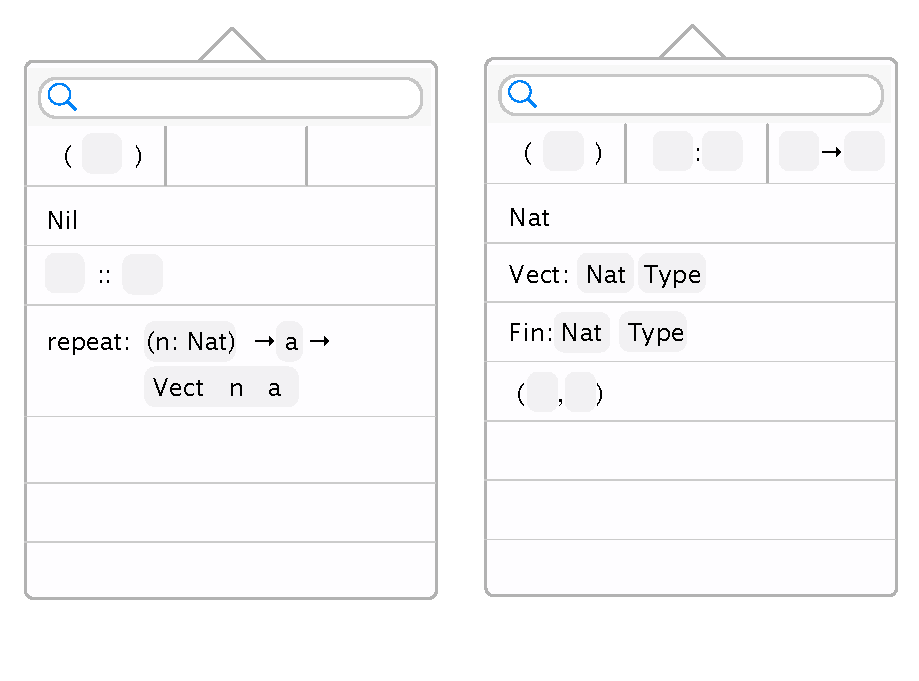
\includegraphics[width=110mm]{diagrams/final_design_popover.pdf}
	\caption{The context popover. Left: How it looks when a \texttt{Vect} is
	expected. Right: How it looks when defining a new type constructor.}
\label{fig:new_design_popover}
\end{figure}

In this design, writing a program would consist of filing a series of holes for terms by choosing applicable functions and constructors from the popover, and only using the virtual keyboard for writing constants, variable names, or searching.
Once a term has been filled, it can be dragged around, and gestures can be used to manipulate it without clashing with text input gestures.
To edit a term, the user can double tap it to bring up the context popover, with any new choices replacing the old choice.
This design means there would be no risk of the user making syntax errors, but on the other hand there would be less freedom to approach the programming task in the way the user prefers, which will be addresed in Section~\todo{Ref}.

The content of the context popover can be sorted by both the frequency of use of a specific item, as well as locality, such that functions defined in the same file are given precedence over library functions.
Getting this heuristic right would require testing with users.

Populating the context popover would require a feature not currently available in the Idris slave mode: searching by type.
For the popover to work, we would have to be able to ask Idris for all constructors and functions that have some specific type, for example \texttt{Nat -> String}.
We believe this to be a feasible extension to Idris. 

\section{Managing Program Structure}
\label{subsec:managing_program_structure}
% F4, F5, Re7, Re13, Re14
Figure~\ref{fig:new_data_declaration} shows two top-level declarations
where none of them are in focus. 
In this state the programmer can get a clear overview of the program without any clutter. 
Tapping anywhere on a declaration takes the user to the state seen in Figure~\ref{fig:new_design_data_in_focus}, where the elements of the declaration are bigger and easier to tap.
The check mark button removes focus from the current declaration and should help mitigate \textbf{I4} by giving the user a clear way to indicate that he is done with editing, following \textbf{Re7}.
Tapping other top-level declarations will switch the current editable declaration to non-editable and switch the tapped top-level declaration to editable.

\begin{figure}
	\centering
		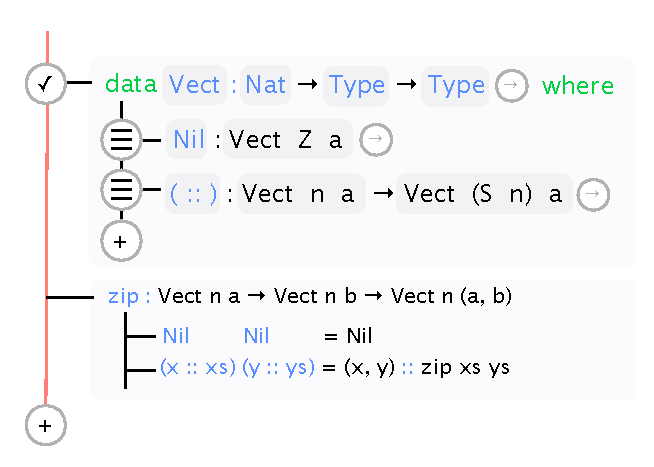
\includegraphics[width=100mm]{diagrams/final_design_top_dec_in_focus.pdf}
	\caption{The new design with a data declarations in focus. The code becomes
	bigger and easier to tap}
\label{fig:new_design_data_in_focus}
\end{figure}

\begin{figure}
	\centering
		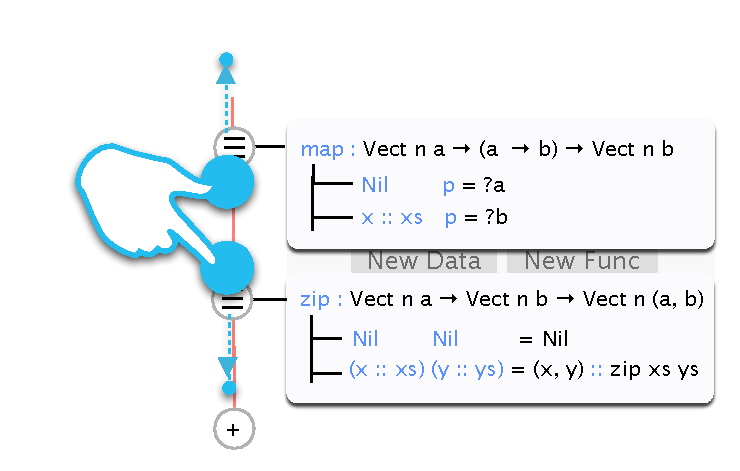
\includegraphics[width=110mm]{diagrams/new_function_reverse_pinch.pdf}
	\caption{When reverse pinching two adjacent handles for top-level
	declarations, a new top-level declaration appears between the old ones.}
\label{fig:new_function_reverse_pinch}
\end{figure}

We have decided to keep our original design for creating new top-level
declarations. Either, the programmer can use the [+] button at the bottom of
the program, or he can reverse-pinch two adjacent top-level declarations to
create a new one between them. This also works for creating constructors
between existing constructors in data declarations.

Now that the representation of a term is no longer overloaded with conflicting
gestures, we can incorporate drag-to-rearrange. Figure\ref{fig:design_drag_to_garbage}
shows an example of this behavior. When the user begins to drag a term, it pops
out of its current position, and can be rearranged with other terms on the same
line. Also, while the user is dragging the term, a trash icon appears in the
upper right corner of the screen, to indicate that it can be deleted. Experienced users can flick the term towards the trash icon, whereas novice users will just drag it.
Clauses in functions and constructors for data can also be deleted in this way, thus fulfilling \textbf{F-4} and \textbf{F-5}.

\begin{figure}
	\centering
		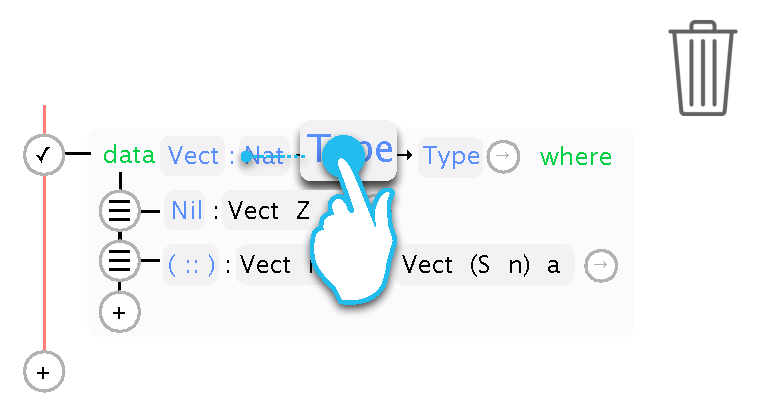
\includegraphics[width=110mm]{diagrams/design_drag_to_garbage.pdf}
	\caption{When reverse pinching two adjacent handles for top-level
	declarations, a new top-level declaration appears between the old ones.}
\label{fig:design_drag_to_garbage}
\end{figure}

\section{Data Declarations}
\label{subsec:new_design_data_dec}
Due to the many issues uncovered concerning the Epigram-inspired data declarations (described in \textbf{I1}, \textbf{I6} in Section~\ref{sec:first_issues} and Section~\ref{sec:second_issues}, respectively), and our failure to improve the situation substantially, we decided to try a more traditional approach to data declarations.

\begin{figure}
	\centering
		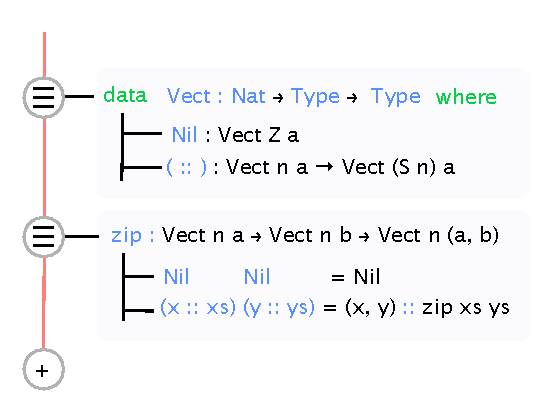
\includegraphics[width=100mm]{diagrams/final_design_nothing_in_focus.pdf}
	\caption{The new data declaration, along with the familiar function declaration.}
\label{fig:new_data_declaration}
\end{figure}

The new data declaration is shown in Figure~\ref{fig:new_data_declaration}.
It is very reminiscent of how data is declared in textual Idris, and in other functional programming languages.
It is our hope that this design will make it easier to read and write data declarations for users not familiar with the interface. This change obviates \textbf{Re8} and \textbf{Re9}, and potentially solves \textbf{I1} and \textbf{I6}.

\section{Function Declarations}
\label{subsec:new_design_function_dec}
The function declarations work much the same way as the data declarations
except for the extra support for initial pattern match creation, case splitting
and meta variable solving.

The initial pattern match creation is still done by pressing the [+] button to
add a new clause. Case splitting can no longer be done by double tapping a
term, as this would toggle it to edit mode. Instead, the user drags the term
down and a new clause appears like it can be seen in Figure~\ref{fig:case_splitting}.

\begin{figure}
	\centering
		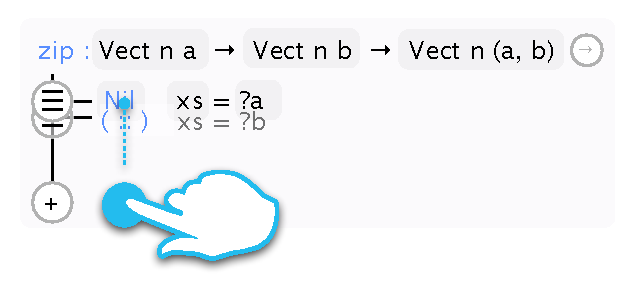
\includegraphics[width=100mm]{diagrams/design_case_splitting.pdf}
	\caption{Case splitting is done by dragging a term down until a new clause
	appears.}
\label{fig:case_splitting}
\end{figure}

Meta variable solving is managed in an even simpler way. If a term starts with
a question mark like in Figure~\ref{fig:case_splitting} then a single tap will
tell the compiler to try and automatically solve the meta variable. Double
tapping it will as always make the term toggle to edit mode.

\section{Virtual Keyboard}
%F-10
\label{subsec:virtual_keyboard}
We have also extended the virtual keyboard with a shortcut bar, inspired by the one in Textastic, as can be seen in Figure~\ref{fig:design_keyboard}.
Each button in the bar can hold several symbols.
To select a specific symbol, the user first touches the button, then swipes in the direction of the desired symbol, and lets go.
For example, to select the plus symbol, the user would touch the leftmost button in the bar, then swipe left.
The bar also features a button to the far right that lets the user add a new argument when specifying types. 
This design solves requirement \textbf{F-10}. 

\begin{figure}
	\centering
		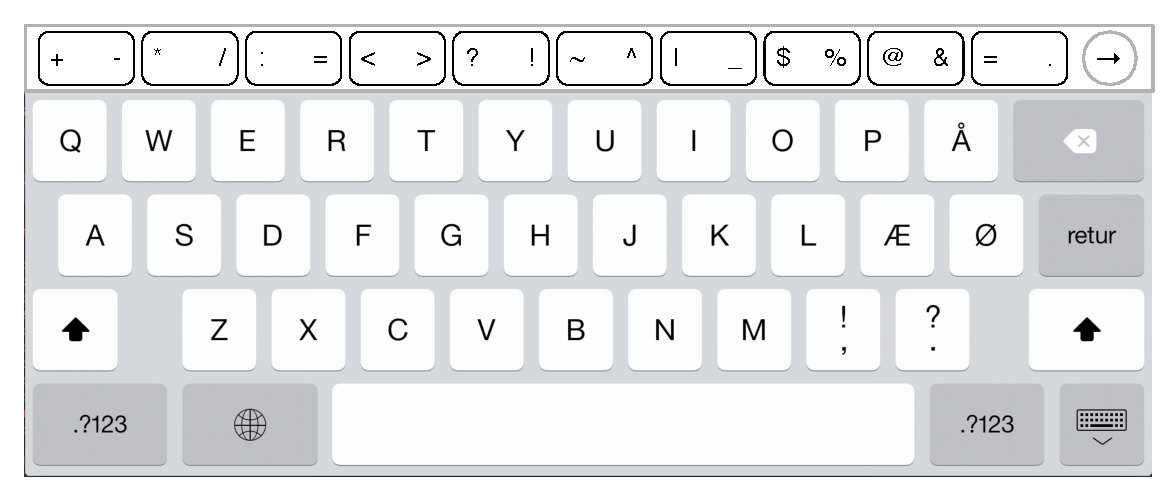
\includegraphics[width=115mm]{diagrams/design_keyboard.pdf}
	\caption{The Textastic-inspired keyboard with common symbols.}
\label{fig:design_keyboard}
\end{figure}

\section{Error Handling}
% U-5
\label{subsec:error_handling}
So far our usability tests have not focused on error handling at all, but in this iteration it is time to begin focusing on this important part of the edit-compile-test cycle.
We propose that errors are indicated by a red background on the term that contains an error. 
Tapping on this term will bring up the context popover that will indicate the error.
For example, say the user has written the term \texttt{foo (bar a b) 2}.
Somewhere else, \texttt{foo} is redefined so the second argument is no longer needed.
In this case, the \texttt{2} would be highlighted in red, and the user can then flick it to the trash, as described above.
It should be noted that the error reporting can only be as good as the error messages are in Idris.
If Idris can not identify the exact placement of the error, it might be necessary to mark a larger area as erroneous, and let the user find the exact problem by reading the error message.
This feature solves \textbf{U-5}.

\section{Third Usability Iteration}
\todo{Rename all usability sections to "Number Usability Test"}
\label{subsec:third_usability_test}
With this new design we feel that the user interface has reached a maturity
level where it is important to focus on the server-side for a while. In the
next usability test, the solution's edit-compile-test cycle should be tested to
a larger extent, and that requires a working back-end. The following usability
test cases assume that we have a working prototype with the new design
implemented as well as a working server that can serve compilation results.

The participants of the usability test should again be a mix of programmers
that are new to the platform and some that are not. Other than that, they
should be screened in the same way as in our second usability test (Section
\ref{sec:SecondUsabilityTest}).

What we specifically wish to test in this next usability test is:

\begin{enumerate}
	\item The flow when declaring new data types and functions. This includes the auto-completion feature and the context popover
	\item The understandability of the way we now declare data types
	\item The focus system, where only one top-level declaration is in focus at a
	time. Can users maneuver in and out of declarations in a fairly easy way?
	\item Editing right-hand sides that have already been added.
	\item Deleting terms by flicking them and rearranging them by dragging.
	\item Deleting top-level declarations, clauses, and constructors
\end{enumerate}

It does not make sense to draw up an exact usability test plan like the ones we have made in previous usability
at this point. We would need to have a working version of the solution before a precise test plan can be made. Also, the few points listed above could easily amount to more than 10 tasks, which is more than can be completed in an hour with a participant. For this reason we would have to prioritize the focus of the test, and that can only be done when we have the new solution in our hands and decide what features we are most confident about. 
